\section{Anforderungen}
Für den Bachelorarbeit wurden die Anforderungen bereits in dem Fachmodul definiert.
\subsection{Anforderungen}
\label{sec:anforderungen}
A1. Es soll möglich sein, die Haustüre durch ein Signal zu öffnen. 
\\
\\
A2. Es soll möglich sein, ein Videosignal von der Aussensprechstelle zum Client zu streamen. 
\\
\\
A3. Es soll möglich sein, ein Audiosignal zwischen der Aussensprechstelle und der Client App bidirektional zu streamen. 
\\
\\
A4. Ein digitaler Bildschirm zeigt die Informationen der Bewohner (Name, Vorname, usw) an der Aussensprechstelle an. 
\\
\\
A5. Nach einem Stromunterbruch soll die Anlage automatisch wieder Starten und Funktionsbereit sein. 
\\
\\
A6. Den Datenverkehr zwischen den Endknoten muss Verschlüsselt sein. 
\\
\\
A7. Die Komponenten sollten zwischen -20C und +40C funktionsfähig sein. 
\\
\\
A8. Die Komponenten sollten auch im Fall hoher Feuchtigkeit funktionsfähig sein. (80\%) 
\\
\\
A9. Die Kamera für das Videosignal muss eine Auflösung von mind. 1280x720 Pixel aufweisen.  
\\
\\
A10. Die Materialkosten pro Aussensprechstelle sollten 400.- nicht überschreiten. 
\\
\\
A11. Die Aussensprechstelle soll auch mit nasse/bedeckte Hände bedienbar sein. 
\\
\\
A12. Bei der Innenstelle ist es möglich das Mikrofon auszuschalten, um die Übertragung des Audiosignales zu unterdrücken. 

\subsection{Wunschanforderungen}
W1. Die Komponenten sollten die Speisung durch PoE erhalten. 
\\
\\
W2. Die Kamera für das Videosignal muss eine Auflösung von 1920x1080 Pixel aufweisen. 
\\
\\
W3. Verpasste Besuche sollten aufgezeichnet werden und in der Client App in Form von einem Foto und Notifikation sichtbar sein.
\newpage

\section{Lösungskonzept}
\label{sec:lösungskonzept}
Die \cref{fig:hwoverview} zeigt einen Überblick über die verschiedenen Hardwarekomponenten, die für die \gls{turklingelanlage} benötigt werden.
\\
Es werden nun zwei Begriffe erklärt, die in diesem Dokument von grosse Bedeutung sind. Das erste ist die \gls{turklingelanlage}. Damit gemeint ist die Gesamtheit der Komponenten die denn Zusammen den Endprodukt darstellen.
\\
Als \gls{aussensprechstelle} ist die Gesamtheit aller Komponenten des Endproduktes gemeint, als Aussensprechstelle der an der Eingangstüre installierte Mikrocontroller inklusive dazugehörige Module.
\\
Räumlich von der \gls{aussensprechstelle} getrennt befindet sich der Server. Dieser besteht aus einem Mikrocontroller, der als Server im Einsatz steht, aus einem Switch der dazu dient die \gls{aussensprechstelle} mit Strom und Datenverbindung zu versorgen und aus einem Relais welches den Türöffner und die Glocke betätigt.
\begin{figure}[htb!]
	\begin{center}
		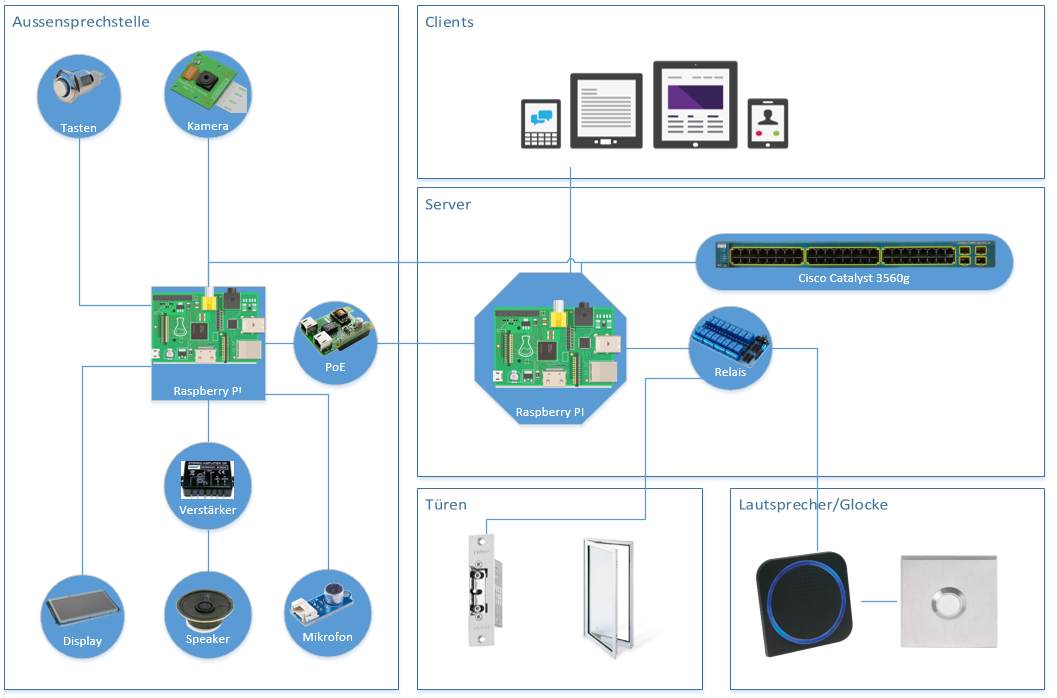
\includegraphics[width=0.95\textwidth]{hwoverview}
		\caption[Hardware Ecosystem]{Hardware Ecosystem}
		\label{fig:hwoverview}
	\end{center}
\end{figure}
Das System besteht aber nicht nur aus Hardware. Das Zusammenarbeiten der Hardware wird von viel Softwareelemente geregelt. Als erstes, wie bereits in der Projektplanung definiert, wird die Hardwareseite der Lösung realisiert. Sobald alle Hardwarekomponenten getestet und auf Kompatibilität geprüft worden sind, wird die Programmierung stattfinden.
\newpage

\section{Hardware}
\label{sec:chapterexample}
\subsection{Komponenten}
Das System wird hardwareseitig grob in zwei Teile unterteilt, den Server und die \gls{aussensprechstelle}.
\\
Die \cref{tbl:SrvHW} und die \cref{tbl:DoorHW} zeigen die benötigten Hardwarekomponenten, welchen an den jeweiligen Stellen eingebaut werden.
\\
Um den Überblick über die Kosten aller Hardwarekomponenten zu behalten, sind hier auch die Preisen aufgelistet. Dabei ist es wichtig sicherzustellen, dass die gesamten Hardwarekosten diejenigen der von der Konkurrenz angebotenen Produkte nicht übersteigen (\seeref{sec:anforderungen} Anforderung A10).
\\
Die Einkaufspreise sind nur Richtpreise, da es sich um Standardkomponenten handelt und die Marktpreise sich ständig und schnell ändern können. Die Summen sind als Kostenschätzung zu betrachten. (Stand Fruhjahr 2017).

\begin{table}[]
	\centering
	\label{my-label}
	\begin{tabular}{l|ll}
		\multicolumn{1}{r|}{} \textbf{Anzahl} & \textbf{Komponente} \hspace{180pt} & \textbf{Preis} 	\\ \hline
		1	&	Raspberry Pi 3 Model B						& 50.-				\\ \hline
		1	&	Raspberry Gehäuse und Netzteil				& 25.-			\\ \hline
		2	&	8-Kanal Relais Modul						& 15.-			\\ \hline
		1	&	\textit{Kleinmaterial}						& 15.-			\\ \hline
		\textbf{Total}	&									& \textbf{140.-}			\\ \hline
	\end{tabular}
	\caption{Server \gls{hw} Komponenten}
	\label{tbl:SrvHW}
\end{table}

\begin{table}[]
	\centering
	\label{my-label}
	\begin{tabular}{l|ll}
		\multicolumn{1}{r|}{} \textbf{Anzahl} & \textbf{Komponente} \hspace{180pt} & \textbf{Preis} 	\\ \hline
		1	&	Raspberry Pi 3 Model B		   				& 50.-			\\ \hline
		1	&	4" Bildschirm								& 64.-			\\ \hline
		1	&	Raspberry Kamera							& 59.-			\\ \hline
		1	&	\gls{poe} Adapter									& 50.-			\\ \hline
		3	&	Schalter									& 25.-			\\ \hline
		1	&	Mikrophon									& 12.-			\\ \hline
		1	&	Lautsprecher								& 9.-			\\ \hline
		1	&	Audio Verstärker							& 10.-			\\ \hline
		1	&	\textit{Kleinmaterial / Gehäuse}			& 50.-			\\ \hline
		\textbf{Total}	&									& \textbf{329.-}			\\ \hline
	\end{tabular}
	\caption{Aussensprechstelle \gls{hw} Komponenten}
	\label{tbl:DoorHW}
\end{table}

\subsection{Stromspeisung}
\label{sec:poe}
Ein Ziel unserer Lösung ist die Installationskosten zu senken und die Montage zu vereinfachen. Aus diesem Grund war für unsere Lösung wichtig, \gls{poe} zu verwenden. In modernen Haushalte werden meistens Ethernet Verkabelungen verlegt und dank PoE ist nur noch ein Kabel, welches Strom und Konnektivität gewährleistet, notwendig.
\\
\\
Zusätzlich benötigt das System noch eine Leitung die den Türöffner steuert.
Auch diese Endinstallation kann vereinfacht werden wenn man, anstatt ein dediziertes Kabel zwischen Server und Türöffner einzuziehen,  zwei Drähte des bereits installierten Ethernet Kabels verwendet.
\\
\\
Für den Projekt verwendete Cisco Catalyst 3560g, welcher für den \gls{poe} Stromversorgung zuständig ist, verwendet die Phantomspeisung oder Mode A \cite{poe}. Das heisst, dass die mit der Datenübertragung belegten Drähte mit der Stromversorgung überlagert werden. Dies ist möglich da die Frequenz der Elektrizität 50 Hz beträgt und die der Datenübertragungen im Bereich von 10-100MHz liegt.
\\
Bei einere zukünftige Beschaffung von ein aktuellere Switch muss speziell auf die Stromspeisungstyp (Phantom/Spare Pairs Speisung) geachtet werden.

\begin{figure}[htb!]
	\begin{center}
		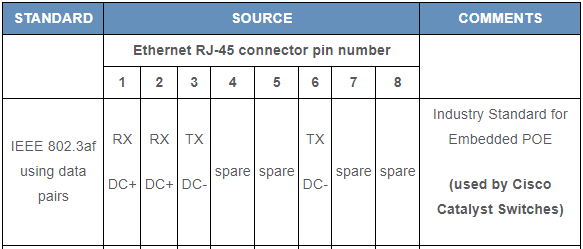
\includegraphics[width=0.89\textwidth]{CatalystPoEpinouts}
		\caption[Catalyst Pinouts]{Catalyst 3560g \gls{poe} Pinbelegung}
		\label{fig:catalystPinouts}
	\end{center}
\end{figure}

Wie im \cref{fig:ethernetBelegung} dargestellt werden die Adern 7 und 8 dazu verwendet um den Türöffner zu betätigen. Aus den 3 verbliebenden Adernpaaren kann maximal die Ethernetkategorie 100BASE-T erreicht werden. Da aber \gls{webrtc} eine erhebliche kleinere Bandbreite in Anspruch nimmt, stellt es für die \gls{aussensprechstelle} kein Hindernis dar.
\\
Durch eine Messung auf die Interface des Switch, an welchem die \gls{aussensprechstelle} angeschlossen ist, konnte die exakte Bandbreite festgestellt werden. Die Messung wurde mit ein Leistungsfähiger Prozessor durchgeführt. Somit wird verhindert dass die Auflösung des Videoübertragung von den Raspberry gedrosselt wird.(Problematik wird im Abschnitt \ref{ssec:alternative} erläutert)
Mit eine hochauflösende Videoübertragung, wurde auf den Interface eine Datenübertragungsrate von 551Kbit/s festgestellt. Die detaillierte Resultate der Messungen sind im Anhang Abschnitt \ref{ssec:resultate} zu finden.

\begin{figure}[htb!]
	\begin{center}
		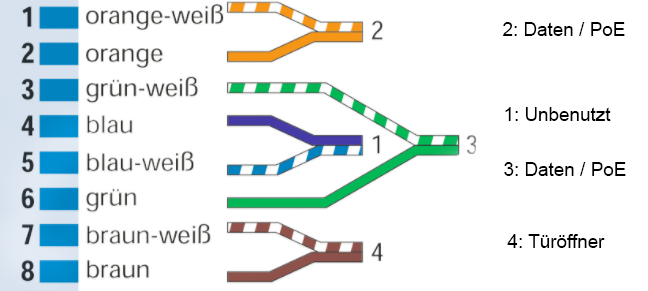
\includegraphics[width=0.89\textwidth]{EthernetPinbelegung}
		\caption[EthernetPinbelegung]{Cat. 7 Ethernet Pinbelegung der \gls{aussensprechstelle}}
		\label{fig:ethernetBelegung}
	\end{center}
\end{figure}



\subsection{Server}
\label{sec:chapterexample}
Der Server wird mit einem Relais-Board verbunden um die Gongs und die Türöffner zu bedienen. An dieser Stelle ist die Hardwarekonfiguration sehr einfach. Mit der aktuellen Hardwarekonfiguration könnten bis 8 Wohnungen und 8 Aussensprechstellen angeschlossen werden. Die \cref{fig:pipins} und die \cref{fig:boardpins} zeigen die Pinbelegung auf dem Pi und auf dem Relais-Board. Die \cref{tbl:pinroutes} zeigt wie die verschiedenen Pins miteinander verbunden werden.

\begin{figure}[htb!]
	\begin{center}
		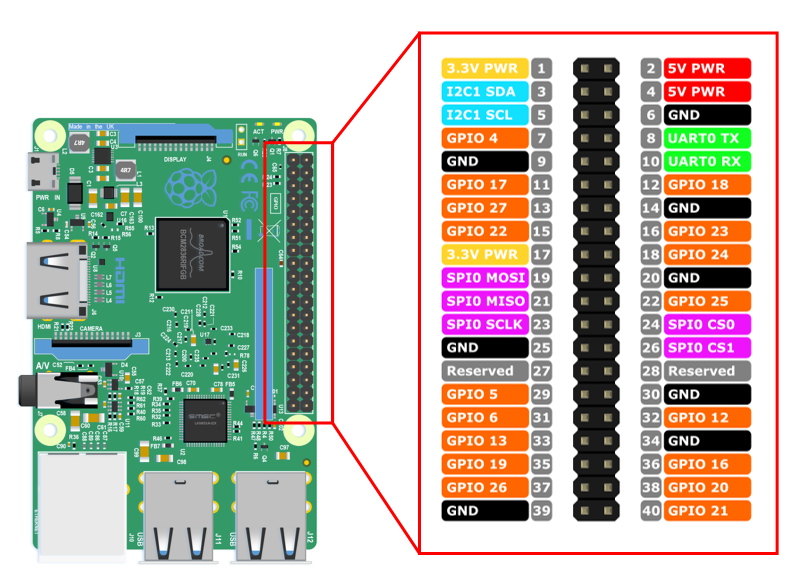
\includegraphics[width=0.8\textwidth]{pipins}
		\caption[EthernetPinbelegung]{Pinbelegung der \gls{aussensprechstelle} (Quelle: http://fablabromagna.org/blog/seminario-iot-presso-corso-di-laurea-ingegneria-e-scienze-informatiche-alma-mater-polo-di-cesena/)}
		\label{fig:pipins}
	\end{center}
\end{figure}

\begin{figure}[htb!]
	\begin{center}
		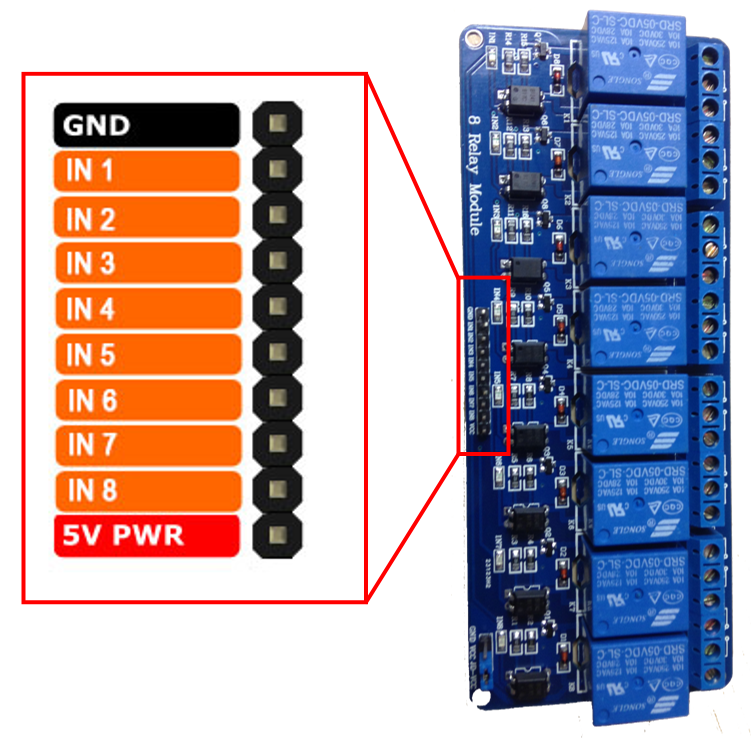
\includegraphics[width=0.55\textwidth]{boardpins}
		\caption[EthernetPinbelegung]{Pinbelegung für das Relais-Modul}
		\label{fig:boardpins}
	\end{center}
\end{figure}

\begin{table}[]
	\centering
	\label{my-label}
	\begin{tabular}{l|ll}
		\multicolumn{1}{r|}{} \textbf{Pi GPIO (PIN)} & \textbf{Relais IN (Board Nr)} & \textbf{Funktion}  \hspace{60pt}	\\ \hline
		GPIO4 (7)	&	IN1 (1)			& Gong WG.1			\\ \hline
		GPIO17 (11)	&	IN2 (1)			& Gong WG.2			\\ \hline
		GPIO27 (13)	&	IN3 (1)			& Gong WG.3			\\ \hline
		GPIO22 (15)	&	IN4 (1)			& Gong WG.4			\\ \hline
		GPIO5 (29)	&	IN5 (1)			& Gong WG.5			\\ \hline
		GPIO6 (31)	&	IN6 (1)			& Gong WG.6			\\ \hline
		GPIO13 (33)	&	IN7 (1)			& Gong WG.7			\\ \hline
		GPIO19 (35)	&	IN8 (1)			& Gong WG.8			\\ \hline
		GPIO18 (12)	&	IN1 (2)			& Türöffner Türe 1			\\ \hline
		GPIO23 (16)	&	IN2 (2)			& Türöffner Türe 2			\\ \hline
		GPIO24 (18)	&	IN3 (2)			& Türöffner Türe 3			\\ \hline
		GPIO25 (22)	&	IN4 (2)			& Türöffner Türe 4			\\ \hline
		GPIO12 (32)	&	IN5 (2)			& Türöffner Türe 5			\\ \hline
		GPIO16 (36)	&	IN6 (2)			& Türöffner Türe 6			\\ \hline
		GPIO20 (38)	&	IN7 (2)			& Türöffner Türe 7			\\ \hline
		GPIO21 (40)	&	IN8 (2)			& Türöffner Türe 8			\\ \hline
	\end{tabular}
	\caption{PIN-Zuweisung zwischen den Server und die Relais Module}
	\label{tbl:pinroutes}
\end{table}


\subsection{Aussensprechstelle}
\label{sec:chapterexample}
Bei der \gls{aussensprechstelle} wird auch ein Raspberry Pi eingesetzt. Hier sind mehrere Zusatzkomponenten notwendig. Die Speisung, wie oben schon erwähnt, erfolgt an dieser Stelle über \gls{poe}. Aus diesem Grund ist ein \gls{poe}-Splitter vorhanden.
\\
Für die Audiowiedergabe sind ein kleiner Lautsprecher und ein Verstärker notwendig. Der Chinch Anschluss des Raspberrys Pi hat eine zu niedrige Ausgangsleistung um den Lautsprecher direkt anschliessen zu können.
\\
Die drei Schalter, die für die Bedienung der \gls{aussensprechstelle} notwendig sind, werden an die \gls{gpio}s des Raspberrys PI angeschlossen. Die \cref{tbl:pinroutesdoor} zeigt die Pinbelegung.

\begin{table}[]
	\centering
	\label{my-label}
	\begin{tabular}{l|ll}
		\multicolumn{1}{r|}{} \textbf{Pi GPIO (PIN)} & \textbf{Schalter} & \textbf{Funktion} \hspace{60pt}	\\ \hline
		GPIO16 (36)	&	Schalter Links		&	Nach Links Scrollen	\\ \hline
		GPIO20 (38)	&	Schalter Mitte		&	Glocke läuten		\\ \hline
		GPIO21 (40)	&	Schalter Rechts		&	Nach Rechts Scrollen		\\ \hline
	\end{tabular}
	\caption{PIN-Zuweisung zwischen den Raspberry PI und die Schalter}
	\label{tbl:pinroutesdoor}
\end{table}

\subsubsection{Problemen}
Während der Zusammenstellung der Aussensprechstelle sind die erste unvorhergesehene Problemen aufgetaucht. Die Audiowiedergabe und Audioaufnahme stellten eine grössere Herausforderung als geplant dar.
\\
\\
\textbf{Audiowidergabe} 
\\
Die grösste Problematik bei der Audiowiedergabe besteht darin, dass die Massen des Raspberrys Pi, des Verstärkers und des Audio-Interface gekoppelt sind. Das führt zu Brummschleifen, die wiederum Störsignale auf dem Audio-Ausgang erzeugen. Um das zu vermeiden, muss an dieser Stelle ein Massentrennfilter eingesetzt werden.
\\
Die Störsignale sind nun fast komplett verschwunden, nur ein winziges Hintergrundgeräusch ist immer noch vorhanden. Um dieses Problem umzugehen, wird ein zusätzliches Relais installiert, welches den Lautsprecherstromkreis bei Nichtnutzung unterbricht.
\\
\\
\textbf{Das Mikrophon}
\\
Das Problem der Audioaufnahme liegt beim Mikrophon selber. Der Raspberry Pi besitzt kein integriertes Audio-Input. Aus diesem Grund wurde ein \gls{usb}-Audio-Interface verwendet. Es hat sich aber herausgestellt, dass es nicht so einfach ist, kostengünstige und qualitatives \gls{usb} Mikrophone zu finden. Die meisten Produkten sind nicht für den Outdoorbetrieb gedacht. Für unseren Prototyp wird das eingesetzte Mikrophon völlig ausreichen, für ein gut funktionierendes Endprodukt sollte man ein besseres Mikrophon einbauen.
\newpage